\chapter{Tiling Problem}
\section{Problem statement}
We are given rod of lenght $N$ and $3$  colored patches of lenght $2,3$ and $4$ and color blue, red and purple respectively. We can apply patches on the rod only if the patch fits completly on te rod. Moreover two patches are not allowed to touch or overlap.

For instanceif we are given a rod of length $5$ the first two arrangements in figure \ref{fig:tiling:example_solution} are valid while the third one is invalid because the purple patch does not fit entirely in the rod.
\begin{figure}
	\label{fig:tiling:example_solution}
	\centering
	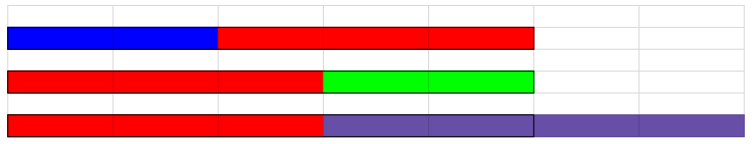
\includegraphics[width=\textwidth]{../problems/tiling_problem/solutions}
	\caption{Three arrangements for the tiling problem.}
\end{figure}

\section{Solution}
This is a classical example of problem solvable by dynamic programming. Let's consider the what happen when we are given a rod of lenght $N \leq 50$.
We can either choose to apply the a patch of size $2$ right from its beginning or ignore the first unit of space of the rod.
In the first case what we are left with is, de facto, a smaller rod of size $N-2$ because all the space used by the first patch is it now not usable anymore.
In the second case we are also left with a smaller rod of $N-1$ because we decided not to use that space. The key idea here is that the problem that we are left with after each of those two cases is exactly of the same kind of the one that we started with, but the rod this time is smaller. 

The second key idea is the realization that there cannot be more than $N$ of those problems because we can get one for each unit of the rod. 

The third key idea is that we can get to solve the subproblem $N-k$ more than one time. For instance we can solve the problem $N-2$ if:
\begin{enumerate}
	\item the blue patch is used
	\item the first unit of space is ignored, leading to a subproblem of size $N-1$ and also for this one the space is ignored.
\end{enumerate}
If we can somehow chache the answer for each of those subproblem then, we can easily avoid recomputing it, thus saving time. 
Fig. \ref{fig:tiling:tree} shows how for instance the subproblem of size $N-4$ is solved at least $4$ times.

The forth idea is that we can consider skipping one unit of space as applying a patch of size one.

Let $S(n)$ be the solution to the problem for a rod of size $n$, we can formalize the previous reasoning by mean of a recurrence relation as in Eq. \ref{eq:tiling:rec_rec}.
\begin{equation}
\label{eq:tiling:rec_rec}
S(n)=\begin{cases}
    \sum_{i \in \{1,2,3,4\}}S(n-i), & \text{if $n\geq0$}.\\
    \infty, & \text{otherwise}.
  \end{cases}
\end{equation}

\begin{figure}
\label{fig:tiling:tree}
\Tree[.$N$ [.$N-1$ [.N-2 ] [.N-3 ] [.N-4 ] [.N-5 ]]
           [.$N-2$ [.N-3 ] [.N-4 ] [.N-5 ] [.N-6 ]]
           [.$N-3$ [.N-4 ] [.N-5 ] [.N-6 ] [.N-7 ]]
           [.$N-4$ [.N-5 ] [.N-6 ] [.N-7 ] [.N-8 ]]
           ]
          \caption{Representation of the first layers of the recursion tree arising from Eq. \ref{eq:tiling:rec_rec}.}
\end{figure}



The following code shows how to implement the idea described above:
\begin{lstlisting}[language=c++, caption="Distinc pair problem. Brute force approach.",label=list:knapexp]
long long ways(const int N, const vector<int>& lengths){
	constexpr int MAXL = 51;
	static long long DP[MAXL]{0};
    
    if(N==0) //as in the recurrence relation
         return 1;
    if(DP[N]>0) //avoid recomputation
        return DP[N];    
    
    long long ans = 0;
    for(const auto l : lengths){
        if(l<=N)
          ans += ways(N-l,lengths);
    }
    DP[N] = ans; //cache the result
    return ans;
}
long long solve(){
	unsigned n;
	cin>>n;
    return ways(n,{1,2,3,4};   
}
\end{lstlisting}






